\chapter{Dynamic Systems and Control}

% Layout
% 

(from introduction)

"Considering that any currency mechanism is absent from this model of sup-
ply and demand is seems reasonable to find a way to include currency in our
model. This leads to the question of what methods should be used to analyze
the properties of currency."

"The fundamental insight that we present is that because currency is a digital
system, the way to approach its analysis is roughly analogous to the way we
approach the analysis and design of other digital systems (the internet being an
interesting case in point), i.e. that we should approach the analysis of currency
as an engineering problem, and in particular the engineering and control of
dynamic systems."

In this chapter we introduce the engineering and control of dynamic systems.

\section{Negative Feedback}

We are looking for a way that we can keep the conditions of the system in some desirable state.
Examples are ... If the system is predictable can use an open system. Many systems, however are not
completely predictable. In many case, despite the unpredictability we can still control the system
to a certain degree. One method is to use a closed system. Another method is to introduce a
sophisticated controller into the loop, such as a human, in combination with the mechanism. Examples
are ...

Adapting \ref{fig:feedback_schema} to the case of a person on a bicycle,

\begin{figure}
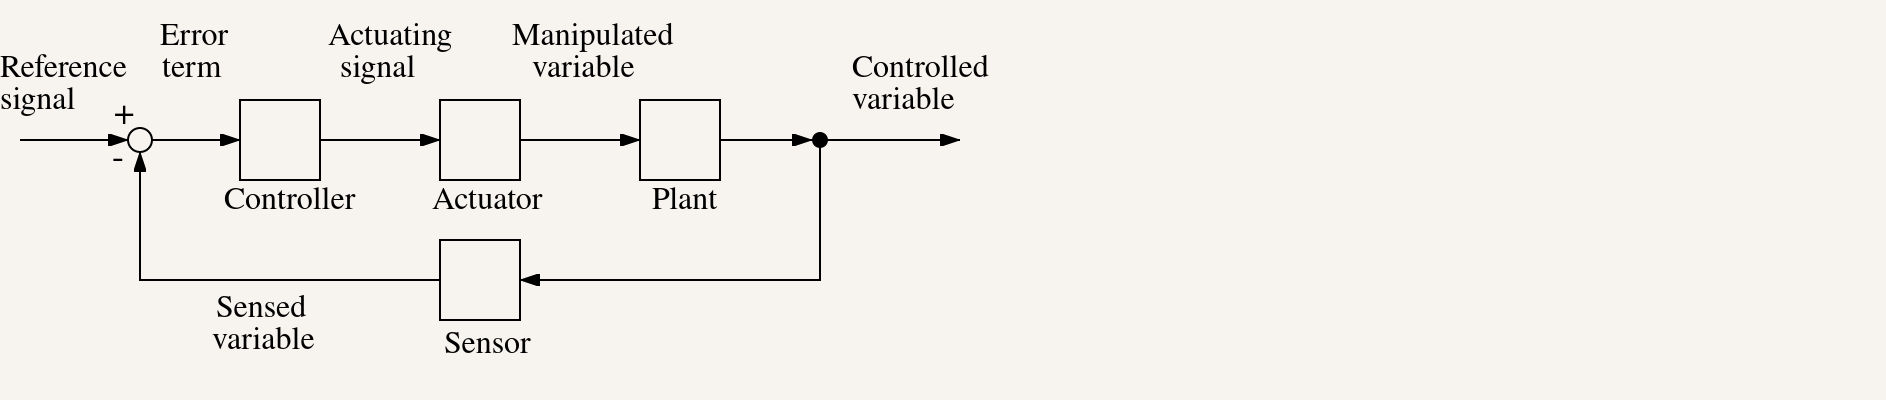
\includegraphics[scale=0.28]{/02/bicycle_feedback_schema}
\caption{Bicycle}
\label{fig:bicycle_feedback_schema}
\end{figure}

\section{History of Control Systems} 

\section{Positive Feedback}

\section{Error Correction}

\section{The Internet}


